\section{Norma em \texorpdfstring{$\mathbb R^n$}{Rn}}

A norma euclidiana em $\mathbb R^n$ associa a cada vetor o seu comprimento euclidiano.

\begin{definition}
    Seja $p=(x_1, \ldots, x_n)$ um elemento de $\mathbb R^n$.
    A \emph{norma}\index{norma}\index{norma euclidiana|see{norma}} de $p$ é definida como:
    \begin{equation*}
        \|p\| = \sqrt{p\cdot p}=\sqrt{x_1^2 + \ldots + x_n^2} = \sqrt{\sum_{i=1}^n x_i^2}.
    \end{equation*}
\end{definition}

Como vimos na seção anterior, se $p\in\mathbb R^n$, então $p\cdot p\geq 0$.
Portanto, a raiz quadrada $\sqrt{p\cdot p}$ está bem definida.

A norma de um vetor $v=(x_1, \ldots, x_n)$ é o comprimento euclidiano do vetor que parte da origem até o ponto $(x_1, \ldots, x_n)$.
Vendo $v$ como um ponto no espaço, sua norma será interpretada como a distância de $v$ até a origem.

\begin{example}
    Temos:
    \[
        \|(3,4)\|=\sqrt{3^2+4^2}=5,
    \]
    \[
        \|(1,-2,2)\|=\sqrt{1^2+(-2)^2+2^2}=3,
    \]
    e, em geral,
    \[
        \|(0,\ldots,0)\|=0.
    \]
\end{example}

Algumas propriedades da norma são as seguintes.
\begin{proposition}\index{norma!propriedades}
    Sejam $v, w \in \mathbb R^n$ e $\alpha \in \mathbb R$. Então:
    \begin{enumerate}[label=(\roman*)]
        \item $\|v\| = 0$ se, e somente se, $v=0$;
        \item $\|\alpha v\| = |\alpha| \|v\|$;
        \item $|v\cdot w| \leq \|v\| \|w\|$ (desigualdade de Cauchy-Schwarz)\index{desigualdade de Cauchy-Schwarz};
        \item $\|v+w\| \leq \|v\| + \|w\|$ (desigualdade triangular)\index{desigualdade triangular}.
    \end{enumerate}
\end{proposition}
\begin{proof}
    Vamos verificar cada uma das propriedades. Escreva $v=(x_1, \ldots, x_n)$ e $w=(y_1, \ldots, y_n)$.
    \begin{enumerate}[label=(\roman*)]
        \item Se $v=0$, então $\|v\|=\sqrt{0^2+\ldots+0^2}=0$. Reciprocamente, se $\|v\|=0$, então $\sqrt{\sum_{i=1}^n x_i^2}=0$.
        Assim, $\sum_{i=1}^n x_i^2=0$.
        
        Como $x_i^2\geq 0$ para todo $i$, segue que $x_i^2=0$ para todo $i$.
        Logo, $x_i=0$ para todo $i$, ou seja, $v=0$.
        \item Temos que $\|\alpha v\| = \sqrt{(\alpha x_1)^2 + \ldots + (\alpha x_n)^2} = |\alpha|\sqrt{x_1^2 + \ldots + x_n^2} = |\alpha| \|v\|$.
        \item Se $w=0$, então a expressão desejada é $0\leq 0$, que é verdadeira.
        Se $w\neq 0$, então, para qualquer que seja o número real $t$, temos que:
        \begin{align*}
            0\leq \|v+tw\|^2 &= (v + tw) \cdot (v + tw) \\
            &= v \cdot v + 2t(v \cdot w) + t^2(w \cdot w) \\
            &= \|v\|^2 + 2t(v \cdot w) + t^2\|w\|^2.
        \end{align*}
        Pondo $t=\frac{-v \cdot w}{\|w\|^2}$, temos que:
        \begin{align*}
            0 &\leq \|v\|^2 - 2\frac{(v \cdot w)^2}{\|w\|^2} + \frac{(v \cdot w)^2}{\|w\|^2} \\
            &= \|v\|^2 - \frac{(v \cdot w)^2}{\|w\|^2}.
        \end{align*}
        Como $\|w\|^2>0$, segue que
        \[
            (v \cdot w)^2 \leq \|v\|^2 \|w\|^2.
        \]
        Portanto,
        \[
            |v \cdot w| \leq \|v\| \|w\|.
        \]
        \item A desigualdade triangular segue da desigualdade de Cauchy-Schwarz:
        \begin{equation*}
            \|v+w\|^2 = (v+w) \cdot (v+w) = \|v\|^2 + 2v \cdot w + \|w\|^2 \leq \|v\|^2 + 2\|v\|\|w\| + \|w\|^2 = (\|v\| + \|w\|)^2.
        \end{equation*}

        Como $\|v+w\|\geq 0$ e $\|v\|+\|w\|\geq 0$, concluímos que
        \[
            \|v+w\|\leq \|v\|+\|w\|.
        \]
    \end{enumerate}
\end{proof}

A relação entre norma e produto escalar pode ser utilizada para decidir-se \emph{ortogonalidade}\index{ortogonalidade}\index{vetores ortogonais|see{ortogonalidade}} entre vetores.
É fato conhecido que vale a recíproca do \emph{Teorema de Pitágoras}\index{Teorema de Pitágoras}: se $\triangle BAC$ é um triângulo, então o ângulo $\angle BAC$ é reto se, e somente se, sendo $a, b, c$ respectivamente as medidas dos segmentos $\overline{BC}, \overline{AC}, \overline{AB}$, temos que $a^2=b^2+c^2$.

\begin{figure}[ht]
    \centering
    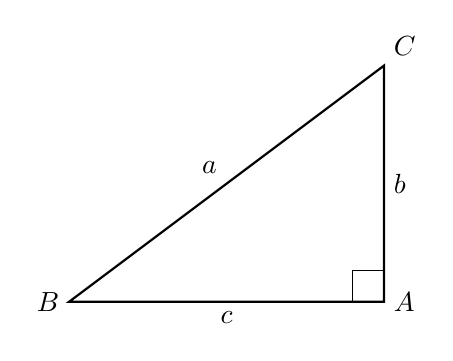
\begin{tikzpicture}
    % Pontos do triângulo
    \coordinate (B) at (0,0);
    \coordinate (A) at (4,0);
    \coordinate (C) at (4,3);

    % Lados do triângulo
    \draw[thick] (B) -- (A) -- (C) -- cycle;

    % Marcação do ângulo reto em A
    \draw (A) ++(-0.4,0) -- ++(0,0.4) -- ++(0.4,0);

    % Nome dos vértices
    \node[right] at (A) {$A$};
    \node[left] at (B) {$B$};
    \node[above right] at (C) {$C$};

    % Lados a, b, c
    \path (B) -- node[above left] {$a$} (C);
    \path (A) -- node[right] {$b$} (C);
    \path (A) -- node[below] {$c$} (B);

    \end{tikzpicture}
    \caption{Triângulo retângulo.}
    \label{fig:triangulo-retangulo}
\end{figure}

    No aspecto vetorial, dados dois vetores $v$ e $w$, perceba que o vetor $v-w=v+(-w)$ pode ser representado como o segmento orientado que une a extremidade de $w$ à extremidade de $v$, conforme ilustrado na Figura~\ref{fig:diferenca-vetores}.

\begin{figure}[ht]
    \centering
    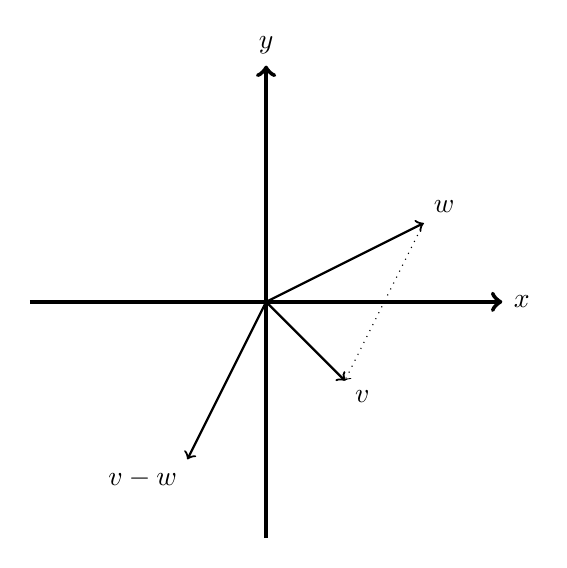
\begin{tikzpicture}
    \draw[->,ultra thick] (-3,0)--(3,0) node[right]{$x$};
    \draw[->,ultra thick] (0,-3)--(0,3) node[above]{$y$};
    % Vetor v
    \draw[->,thick] (0,0) -- (2,1) node[above right]{$w$};
    % Vetor v-w
    \draw[->,thick] (0,0) -- (-1,-2) node[below left]{$v-w$};
    \draw[->,dotted] (2,1) -- (1,-1);
    % Vetor v+w
    \draw[->,thick] (0,0) -- (1,-1) node[below right]{$v$};
    \end{tikzpicture}
    \caption{O vetor $v-w$ como deslocamento da extremidade de $w$ até a extremidade de $v$.}
    \label{fig:diferenca-vetores}
\end{figure}

Motivados pela recíproca do Teorema de Pitágoras, dizemos que dois vetores $v,w\in\mathbb R^n$ são \emph{ortogonais} quando
\[
    \|v-w\|^2=\|v\|^2+\|w\|^2.
\]

\begin{proposition}\index{ortogonalidade!produto escalar}
    Sejam $v, w \in \mathbb R^n$. Então, $v$ e $w$ são ortogonais se, e somente se, $v \cdot w = 0$.
\end{proposition}
\begin{proof}
    Notemos que, no geral:
    \begin{equation*}
        \|v-w\|^2 = (v-w) \cdot (v-w) = v \cdot v - 2v \cdot w + w \cdot w = \|v\|^2 - 2v \cdot w + \|w\|^2.
    \end{equation*}
    Assim, temos que:
    \begin{align*}
        \|v-w\|^2 &= \|v\|^2 + \|w\|^2 \\
        &\iff \|v\|^2 - 2v \cdot w + \|w\|^2 = \|v\|^2 + \|w\|^2 \\
        &\iff -2v \cdot w = 0 \\
        &\iff v \cdot w = 0.
    \end{align*}
\end{proof}

\subsection*{Exercícios}

\begin{exercise}
    Calcule a norma dos seguintes vetores:
    \[
        (3,4),\qquad (1,-2,2),\qquad (2,-1,0,2),\qquad (0,\ldots,0)\in\mathbb R^n.
    \]
\end{exercise}

\begin{exercise}
    Seja $v=(2,-1,2)$.
    Calcule:
    \[
        \|v\|,\qquad \|-v\|,\qquad \|3v\|,\qquad \left\|\frac12v\right\|.
    \]
\end{exercise}

\begin{exercise}
    Determine todos os números reais $\alpha$ tais que, para $v=(1,2,2)$, tenhamos $\|\alpha v\|=9$.
\end{exercise}

\begin{exercise}
    Verifique quais dos seguintes pares de vetores são ortogonais:
    \begin{enumerate}[label=(\alph*)]
        \item $v=(1,2)$ e $w=(2,-1)$;
        \item $v=(1,-1,2)$ e $w=(3,1,-1)$;
        \item $v=(2,0,-1)$ e $w=(1,4,2)$.
    \end{enumerate}
\end{exercise}

\begin{exercise}
    Seja $v=(3,4)$.
    Encontre um vetor $u\in\mathbb R^2$ que tenha a mesma direção e o mesmo sentido de $v$, mas norma igual a $1$.
\end{exercise}

\begin{exercise}
    Seja $v\in\mathbb R^n$ um vetor não nulo.
    Seja
    \[
        u=\frac{1}{\|v\|}v
    \]
    Mostre que $\|u\|=1$.
\end{exercise}

\begin{exercise}
    Sejam $v,w\in\mathbb R^n$.
    Mostre que
    \begin{enumerate}[label=(\alph*)]
        \item $\|-v\|=\|v\|$;
        \item $\|v-w\|=\|w-v\|$;
        \item $\|v+w\|^2=\|v\|^2+2v\cdot w+\|w\|^2$;
        \item $\|v-w\|^2=\|v\|^2-2v\cdot w+\|w\|^2$.
    \end{enumerate}
\end{exercise}

\begin{exercise}
    Sejam $v,w\in\mathbb R^n$.
    Prove que
    \[
        \|v+w\|^2+\|v-w\|^2=2\|v\|^2+2\|w\|^2.
    \]

    Essa igualdade é conhecida como a \emph{identidade do paralelogramo}.
\end{exercise}

\begin{exercise}
    Sejam $v,w\in\mathbb R^n$ vetores ortogonais.
    Mostre que
    \[
        \|v+w\|^2=\|v\|^2+\|w\|^2.
    \]
\end{exercise}

\begin{exercise}
    Use a desigualdade triangular para mostrar que, para todos $v,w\in\mathbb R^n$,
    \[
        \big|\|v\|-\|w\|\big|\leq \|v-w\|.
    \]
\end{exercise}